\documentclass[11pt,a4paper]{article}
\usepackage[utf8]{inputenc}
\usepackage[T1]{fontenc}
\usepackage{amsmath,amssymb}
\usepackage{graphicx}
\usepackage{booktabs}
\usepackage{hyperref}
\usepackage[margin=2.5cm]{geometry}
\usepackage{caption,subcaption}
\usepackage{xcolor,float}
\usepackage{enumitem}
\usepackage{listings}

\lstset{basicstyle=\ttfamily\small, frame=single, breaklines=true}
\hypersetup{colorlinks=true, linkcolor=blue!60!black, citecolor=blue!60!black, urlcolor=blue!60!black}

\title{\textbf{Seating Arrangement Optimizer}\\[4pt]
\large Multi-Objective Evolutionary Approach with Heuristic Seeding and GNN}
\author{}
\date{February 2026}

\begin{document}
\maketitle
\tableofcontents
\newpage

%=================================================================
\section{Problem Statement}
%=================================================================

Given a event with guests organized into \emph{atomic groups}, assign every group to a table such that:
\begin{itemize}[nosep]
    \item No table exceeds capacity $C$ people (typically 10--12).
    \item Related groups sit together (high \emph{cohesion}).
    \item No group is isolated from its tablemates (low \emph{loneliness}).
    \item The number of tables is minimized.
\end{itemize}

\subsection{Guest Tree}

Guests form a rooted tree.  \textbf{Leaf nodes} are guest groups with a size (people count).  \textbf{Internal nodes} are categories (e.g.\ ``bride's side'') with size zero.  Only leaves are assigned to tables.

Figure~\ref{fig:tree_plain} shows our running example: 40 nodes, 22 leaves, 67 people, $C=10$, minimum $\lceil 67/10 \rceil = 7$ tables.

\begin{figure}[H]
    \centering
    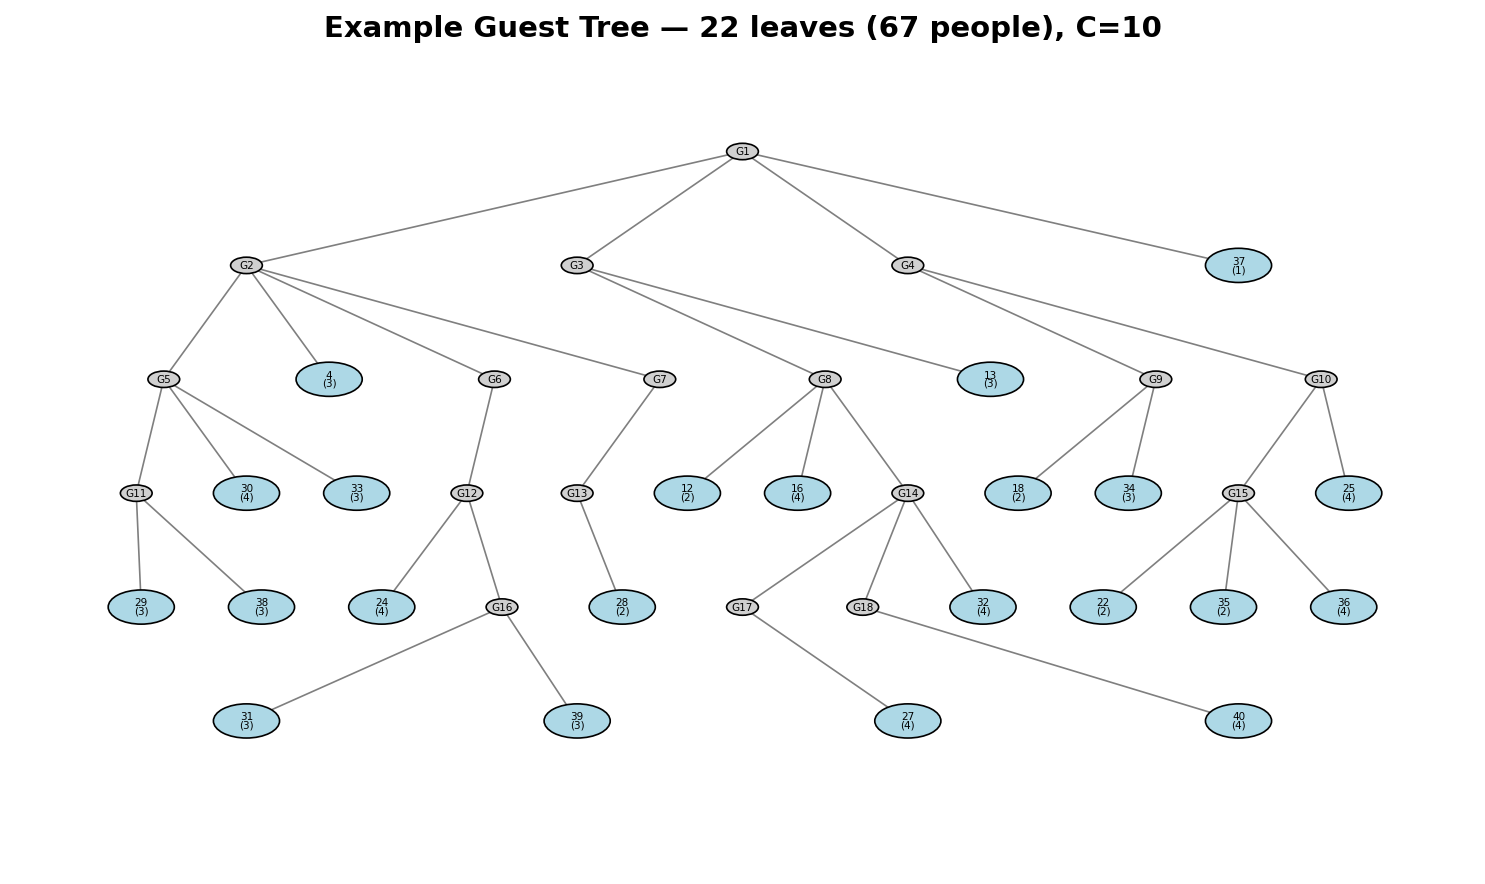
\includegraphics[width=0.75\textwidth]{figures/tree_plain.png}
    \caption{Example guest tree.  Leaf nodes show ``ID (size)''; internal nodes (gray) labeled G1--G18.}
    \label{fig:tree_plain}
\end{figure}

\subsection{Tree Distance}

$\mathrm{dist}(a, b) = \mathrm{depth}(a) + \mathrm{depth}(b) - 2\,\mathrm{depth}(\mathrm{LCA}(a,b))$.
Precomputed via Euler tour + sparse table ($O(n\log n)$ setup, $O(1)$ per query), stored as full $N \times N$ matrix.

\subsection{Objectives (NSGA-II)}

For each leaf $g$ at table $T(g)$:
\begin{align}
    \mathrm{loneliness}(g) &= \min_{h \in T(g),\, h \neq g} \mathrm{dist}(g, h) \\
    \mathrm{cohesion}(g) &= \sum_{h \in T(g),\, h \neq g} \frac{1}{\mathrm{dist}(g, h)}
\end{align}

Minimize: (1) table count $f_1$, (2) penalty $f_2 = \alpha\sum_g \mathrm{loneliness}(g)^p - \sum_g \mathrm{cohesion}(g)$ where $\alpha$ weights loneliness vs cohesion and $p$ penalizes outliers (defaults: $\alpha=2, p=2$).

Table count cap: $N_{\max} = \lceil\text{people}/C\rceil + \Delta$ ($\Delta$ configurable, default 5).

\subsection{Evaluation Metric: Weighted Pareto Score}

$\text{WPS} = \frac{\sum_{k=0}^{\Delta} (\Delta+1-k) \cdot f_2(\text{min\_tables}+k)}{\sum_{k=0}^{\Delta} (\Delta+1-k)}$.
Weights the minimum table count most heavily.  Lower = better.  All tuning uses WPS.

%=================================================================
\section{Initial Population Methods}
\label{sec:init}
%=================================================================

We seed NSGA-II with diverse solutions from five methods.  All examples use the tree from Figure~\ref{fig:tree_plain} with $C=10$, seed=0.  If a method produces more tables than $N_{\max}$ or overflows any table, it falls back to random valid.

\subsection{Random Valid}

\textbf{Algorithm}: iterate leaves in random order; place each at the first table with room; open new table if none fits.

\textbf{Example}: Leaf~29 (size~3) $\to$ Table~4 [3/10].  Leaf~38 (3) $\to$ Table~4 [6/10].  Leaf~35 (2) $\to$ Table~4 [8/10].  Leaf~18 (2) $\to$ Table~4 [10/10].  Leaf~13 (3): full $\to$ Table~3 [3/10].  Leaf~31 (3) $\to$ Table~3 [6/10].  Leaf~24 (4) $\to$ Table~3 [10/10].

Actual tables: \{4,16,39\}=10, \{12,33,34\}=8, \{13,24,31\}=10, \{18,29,35,38\}=10, \{22,25,32\}=10, \{27,30,37\}=9, \{28,36,40\}=10.  \textbf{7 tables, penalty=1269}.  Runtime: 0.7\,ms.

\begin{figure}[H]
    \centering
    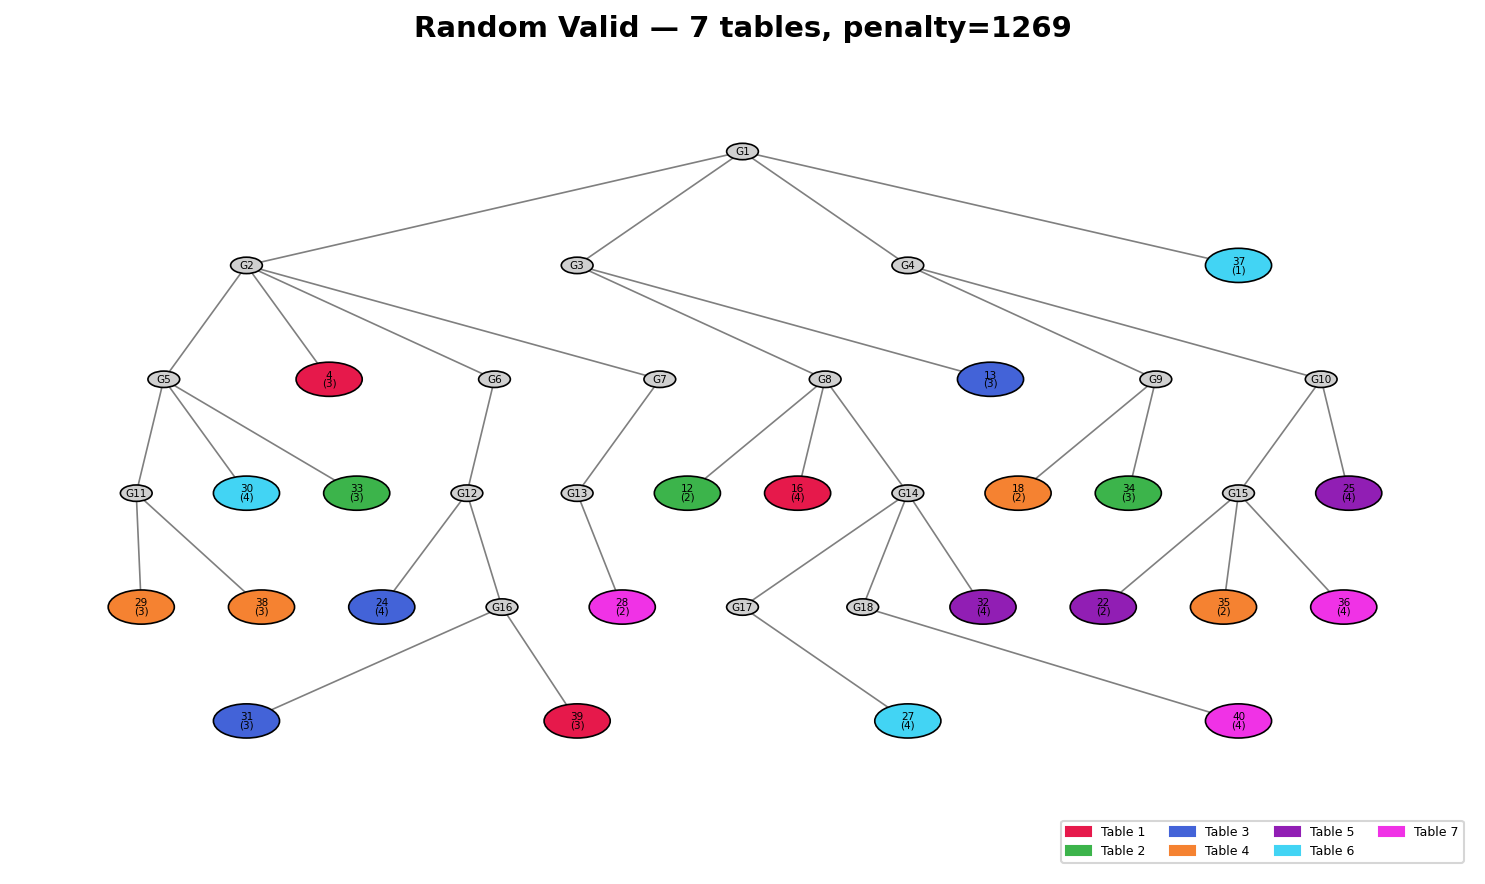
\includegraphics[width=0.65\textwidth]{figures/tree_random.png}
    \caption{Random assignment.  Tables are full but tablemates are unrelated.}
\end{figure}

\subsection{Nearest-Neighbor}

\textbf{Algorithm}: pick random unassigned leaf as seed.  Fill table with closest unassigned leaf (by tree distance) that fits.  Repeat.

\textbf{Example}: Seed leaf~37 (1) $\to$ Table~1.  Closest: leaf~4 (dist=3, size~3) $\to$ [4/10].  Then leaf~13 (dist=3, 3) $\to$ [7/10].  Then leaf~12 (dist=3, 2) $\to$ [9/10].  New seed: leaf~33 (3) $\to$ Table~2.  Closest: leaf~30 (dist=2, 4) $\to$ [7/10].  Then leaf~29 (dist=3, 3) $\to$ [10/10].

Actual tables: \{4,12,13,37\}=9, \{16,28,38\}=9, \{18,22,25,35\}=10, \{24,31,39\}=10, \{27,32\}=8, \{29,30,33\}=10, \{34,36\}=7, \{40\}=4.  \textbf{8 tables, penalty=770}.  Runtime: 9.6\,ms.

\begin{figure}[H]
    \centering
    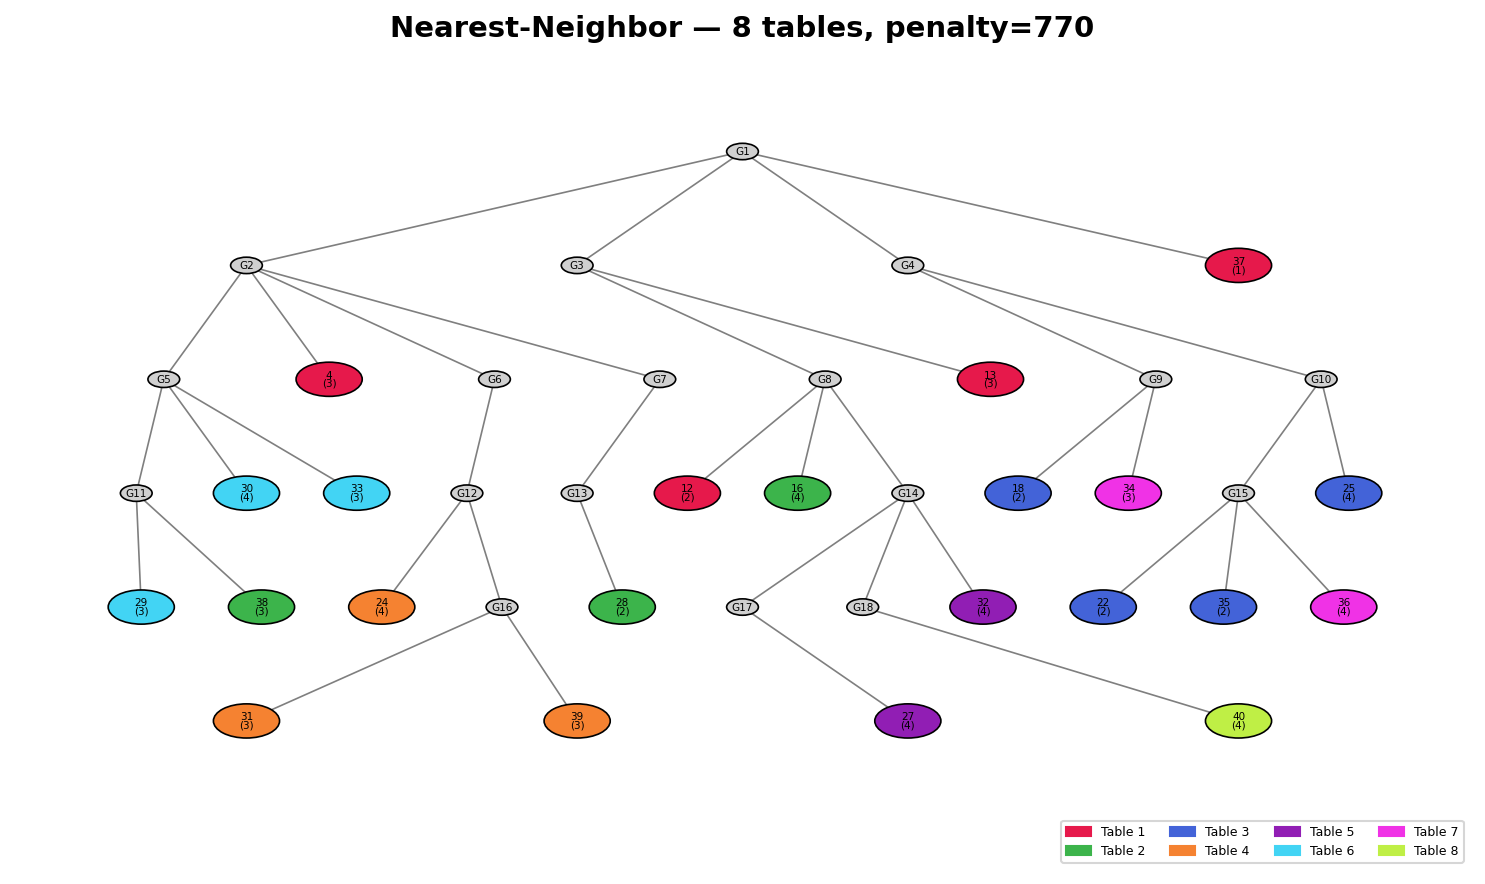
\includegraphics[width=0.65\textwidth]{figures/tree_nearest_neighbor.png}
    \caption{Nearest-neighbor.  Tight clusters but one extra table.}
\end{figure}

\subsection{Greedy Top-Down}

\textbf{Algorithm}: if a node's subtree leaf-total $\leq C$, assign all its leaves to one table.  Otherwise, shuffle children randomly and recurse.

\textbf{Example}: G1 (67 people) $\to$ recurse.  G2 (28) $\to$ recurse.  G11 (6 $\leq$ 10): \{29,38\} $\to$ one table.  Leaf~30 (4) $\to$ own table.  G6 (10 $\leq$ 10): \{24,31,39\} $\to$ one table.

Actual tables after compaction (12): \{4,16\}=7, \{12,28,37\}=5, \{13,33\}=6, \{18,34\}=5, \{22,35,36\}=8, \{24,31,39\}=10, \{25\}=4, \{27\}=4, \{29,38\}=6, \{30\}=4, \{32\}=4, \{40\}=4.  \textbf{16$\to$12 tables, penalty=1213}.  Runtime: 1.5\,ms.

\begin{figure}[H]
    \centering
    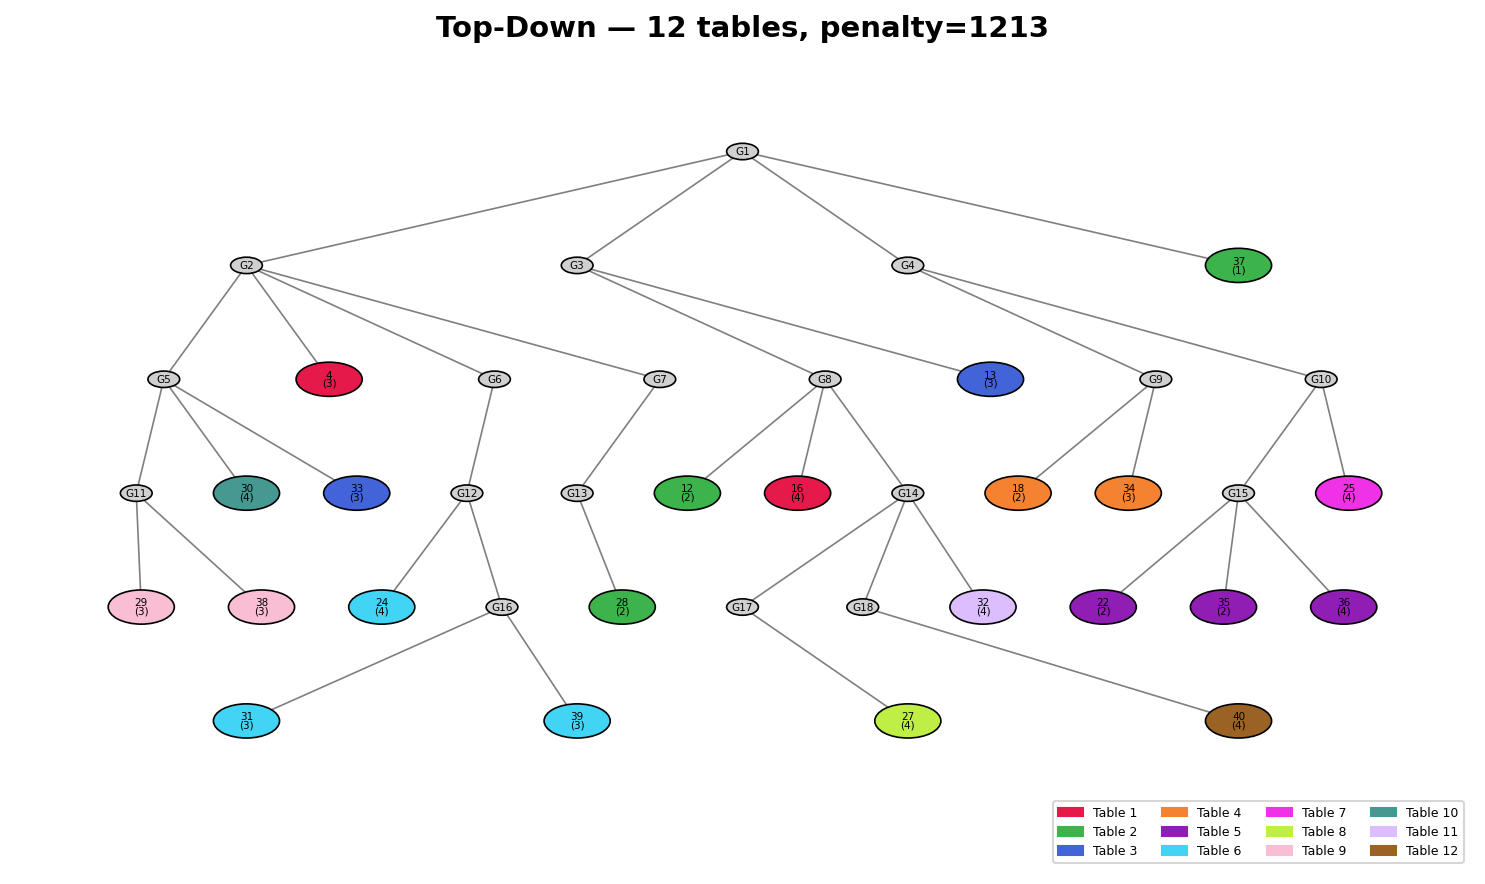
\includegraphics[width=0.65\textwidth]{figures/tree_top_down.png}
    \caption{Top-down.  Subtrees intact but many half-empty tables.}
\end{figure}

\subsection{Bottom-Up Merge}

\textbf{Algorithm}: recursively partition each subtree's leaves into tables (bottom-up), then merge small tables from sibling subtrees via bin-packing with randomized order.  Crosses subtree boundaries.

\textbf{Example}: Starting from the leaves, leaf~12 (size~2) forms its own group.  Moving up, G14 merges leaf~32 (4) with leaf~12 $\to$ \{12,32\}=6.  Then G17 adds leaf~27 (4): \{12,27,32\}=[10/10], a full table.  Similarly, G18 merges leaf~16 (4) with leaf~37 (1) and leaf~40 (4) $\to$ \{16,37,40\}=[9/10].  Top-down would have put leaf~27 and leaf~40 in separate half-empty tables; bottom-up merge packs them together by crossing subtree boundaries.

Actual tables (8): \{4,28,30\}=9, \{12,27,32\}=10, \{13\}=3, \{16,37,40\}=9, \{18,25,34\}=9, \{22,35,36\}=8, \{24,31,39\}=10, \{29,33,38\}=9.  \textbf{8 tables, penalty=442}.  Runtime: 1.0\,ms.

\begin{figure}[H]
    \centering
    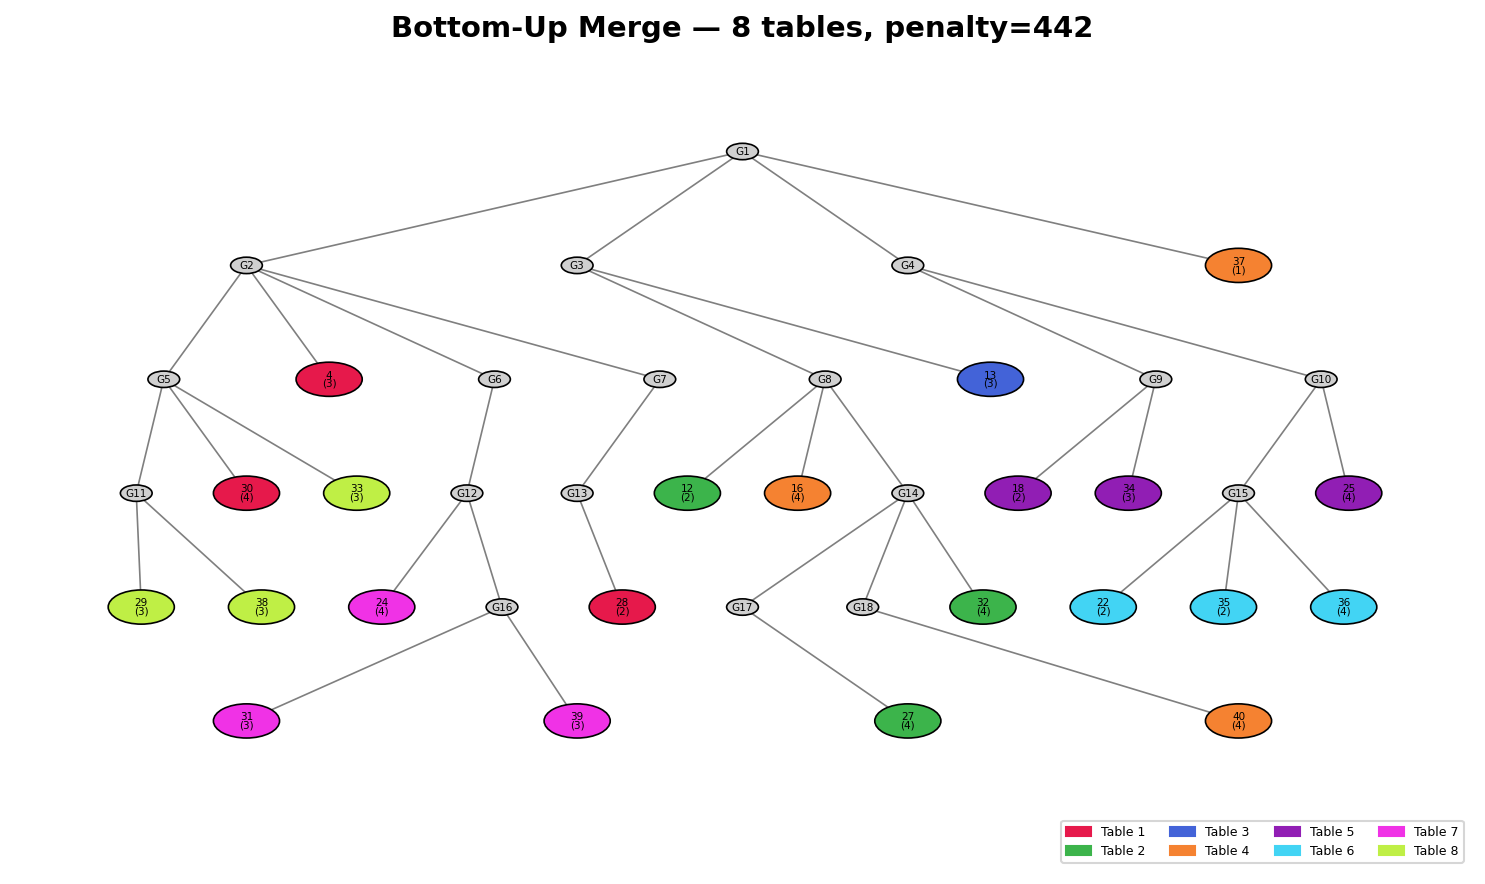
\includegraphics[width=0.65\textwidth]{figures/tree_bottom_up_merge.png}
    \caption{Bottom-up merge.  Crosses subtree boundaries for better packing.}
\end{figure}

\subsection{GNN (Graph Neural Network)}

\textbf{Architecture}: 3-layer GCN with 4 structural features per node (depth, size, is\_leaf, subtree\_people\_fraction).  Produces 32-dim embeddings, trained via contrastive loss: leaves that share a table in the EA's best min-table solution are pulled together in embedding space, while leaves at different tables are pushed apart.  Assignments via nearest-neighbor clustering using blended distance: $d = 0.8 \cdot d_{\text{tree}} + 0.2 \cdot d_{\text{embedding}}$.

\textbf{Example}: Actual tables (8): \{4,12,13,37\}=9, \{16,28,38\}=9, \{18,22,25,35\}=10, \{24,31,39\}=10, \{27,32\}=8, \{29,30,33\}=10, \{34,36\}=7, \{40\}=4.  \textbf{8 tables, penalty=770} (identical to nearest-neighbor on this tree).  Runtime: 14.7\,ms.

\begin{figure}[H]
    \centering
    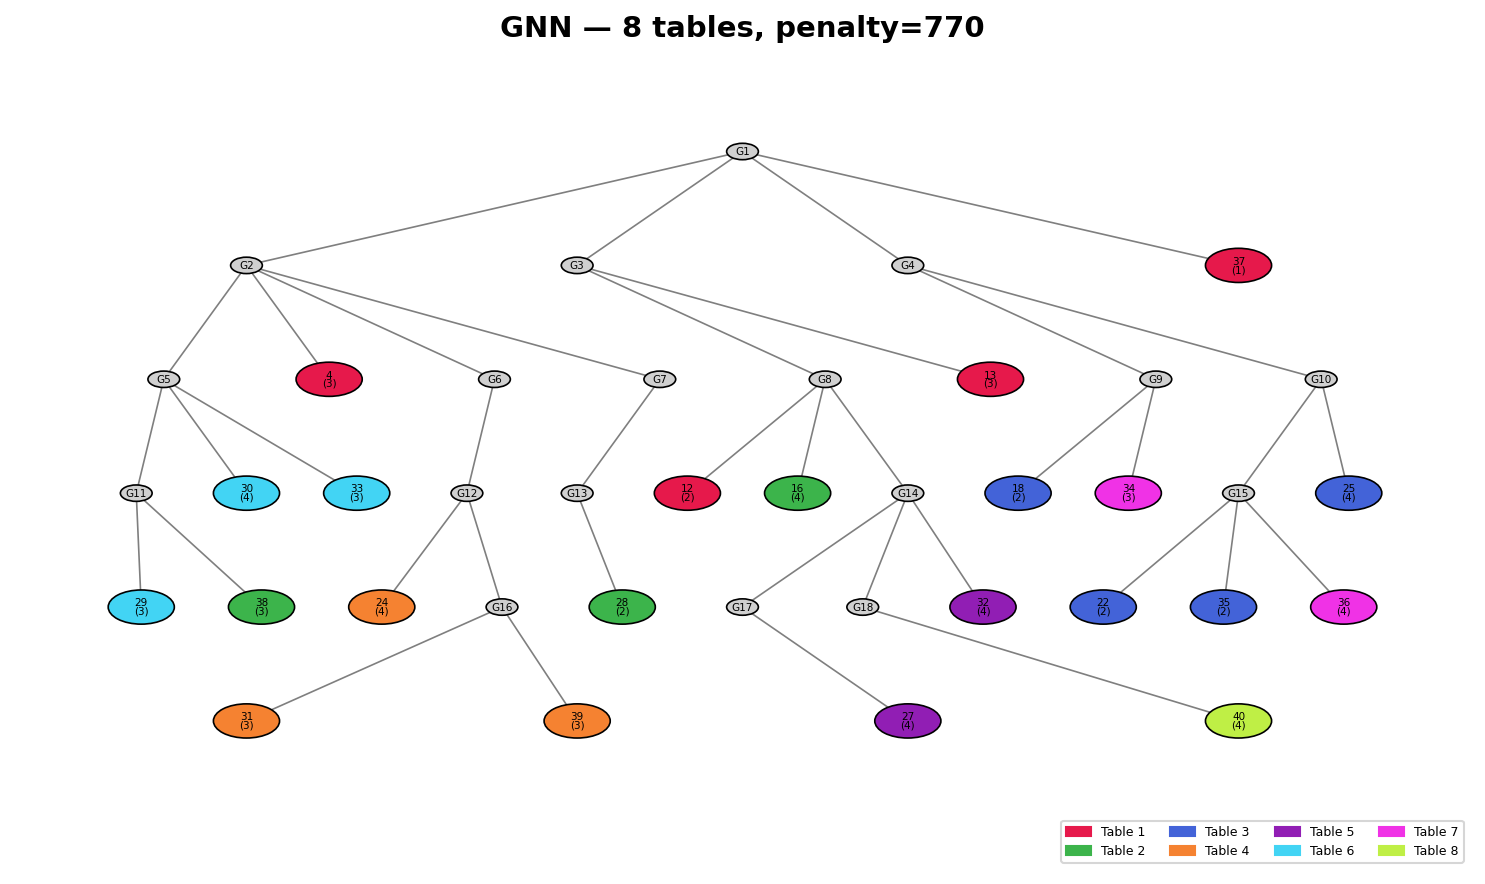
\includegraphics[width=0.65\textwidth]{figures/tree_gnn.png}
    \caption{GNN assignment.  Learned embeddings produce clusters similar to nearest-neighbor.}
\end{figure}

\subsection{Largest-First Nearest-Neighbor}

\textbf{Algorithm}: pick the largest unassigned leaf, start a new table.  Fill by repeatedly choosing the largest remaining leaf that fits, breaking ties by closest tree distance to current table members.  Repeat until all leaves are assigned.

This is a bin-packing heuristic: by placing large groups first, it avoids the fragmentation that leaves small gaps unfillable.  On hard instances (large groups, tight capacity), it consistently reaches the theoretical minimum table count where other initializers cannot.

\textbf{Hard test case} (81 leaves, 366 people, $C=10$, min=37 tables): \texttt{largest\_first\_nn} reaches 37 tables in 50/50 runs.  \texttt{nearest\_neighbor}: 0/50.  \texttt{bottom\_up\_merge}: 0/50.  Without this initializer in the EA population, the optimizer converges to 38 tables because no individual in the initial population ever has 37.

\subsection{Compaction}

All initializers are followed by compaction: greedily merge smallest table pairs until within $N_{\max}$.  If compaction cannot reach $N_{\max}$ without overflowing tables, the method falls back to random valid.  This affects top-down and bottom-up merge on large trees where subtrees exceed $C$.

%=================================================================
\section{Evolutionary Operators}
%=================================================================

\subsection{Mutation}

\begin{table}[H]
\centering
\begin{tabular}{lcp{8cm}}
\toprule
\textbf{Operator} & \textbf{Default} & \textbf{Description} \\
\midrule
Random swap & 40\% & Swap two leaves from different tables if both remain valid. \\
Random move & 40\% & Move one leaf to a different table if it fits. \\
Split table & 5\% & Split a table into two randomly.  Only if count $< N_{\max}$. \\
Merge tables & 5\% & Merge two smallest tables if combined $\leq C$. \\
Nearest-neighbor move & 10\% & Move a leaf to the table of its closest tree neighbor. \\
\bottomrule
\end{tabular}
\end{table}

\subsection{Crossover with Smart Fragment Repair}

Subtree-swap: take leaf assignments from parent~A for a random subtree, rest from parent~B.  Then redistribute members of small fragmented tables ($<50\%$ full) to other tables by best cohesion.

\textbf{Example}: Parent~A (bottom-up merge, 8 tables, penalty=442) and Parent~B (random, 7 tables, penalty=1269).  Subtree rooted at node~17 with leaves \{27,32,40\}:

\begin{enumerate}[nosep]
    \item \textbf{From Parent~A}: leaves 27,32 were at A's Table~2 \{12,27,32\}=[10/10]; leaf~40 at A's Table~4 \{16,37,40\}=[9/10].
    \item \textbf{From Parent~B}: other 19 leaves keep B's assignments.  B's Table~5 \{22,25,32\}=10 loses leaf~32 $\to$ \{22,25\}=6 (fragment).  B's Table~7 \{28,36,40\}=10 loses leaf~40 $\to$ \{28,36\}=6 (fragment).
    \item \textbf{Smart repair}: fragments $<50\%$ full are redistributed.  Leaf~40 (from A) now sits with \{30,37\} forming \{30,37,40\}=9.  Fragments \{22,25\} and \{28,36\} remain as small tables since no room elsewhere.
    \item \textbf{Result}: Child has 8 tables, penalty=1046 (between parents).
\end{enumerate}

Child tables: \{4,16,39\}=10, \{12,33,34\}=8, \{13,24,31\}=10, \{18,29,35,38\}=10, \{22,25\}=6, \{27,32\}=8, \{28,36\}=6, \{30,37,40\}=9.

%=================================================================
\section{GNN Architecture and Training}
%=================================================================

\subsection{Architecture}
\begin{lstlisting}
Input:  4 structural features per node (depth, size, is_leaf, subtree_people_fraction)
GCN Layer 1: 4 -> 64, ReLU
GCN Layer 2: 64 -> 64, ReLU
GCN Layer 3: 64 -> 32 + LayerNorm (embedding)
\end{lstlisting}

The GNN takes only tree-structural features as input.  All four are normalized: depth by max depth, size by table capacity $C$, is\_leaf as binary, and subtree people fraction by total guest count.

\subsection{Training}

\textbf{Data generation}: 1,500 synthetic trees (30--1000 nodes, yielding 13--495 leaves) with randomized table capacities $C \in \{8, 10, 12\}$.  For each tree, a short EA run (pop=40, 40 generations) produces a target assignment---the Pareto-optimal solution with the \emph{lowest penalty at the minimum table count}.  Trees with fewer than 10 leaves are discarded.  Data generation is parallelized across all available CPU cores.

\textbf{Loss}: margin-based contrastive loss over leaf embeddings.  For each pair of leaves $(i, j)$:
\begin{itemize}[nosep]
    \item \textbf{Same table}: pull together---$\ell_{\text{same}} = d(e_i, e_j)^2$
    \item \textbf{Different tables}: push apart with margin $m=3$---$\ell_{\text{diff}} = \max(0, m - d(e_i, e_j))^2$
\end{itemize}
Total: $\mathcal{L} = \frac{\sum_{\text{same}} \ell_{\text{same}}}{|\text{same}|} + 0.5 \cdot \frac{\sum_{\text{diff}} \ell_{\text{diff}}}{|\text{diff}|}$.  The 0.5 weight on the repulsive term ensures the network prioritizes pulling same-table leaves together over pushing different-table leaves apart, compensating for the far more numerous different-table pairs.

\textbf{Optimization}: Adam ($\text{lr}=5 \times 10^{-4}$, weight decay $10^{-5}$), cosine annealing over 200 epochs, gradient clipping at norm 1.0.  Best model (by average loss) is checkpointed.

\subsection{From Embeddings to Tables}

Blended distance: $d_{\text{combined}} = (1-\alpha) \cdot d_{\text{tree}}/\max d_{\text{tree}} + \alpha \cdot d_{\text{emb}}/\max d_{\text{emb}}$ with $\alpha=0.2$.  Then greedy nearest-neighbor clustering using $d_{\text{combined}}$: pick a random unassigned leaf as seed, repeatedly add the closest fitting leaf, open a new table when full.

The low $\alpha$ means tree distance dominates---the GNN embeddings act as a tiebreaker when two leaves are equidistant in the tree.  Higher $\alpha$ degrades table-count packing: at $\alpha \geq 0.3$ the initializer rarely achieves the minimum table count.

\subsection{Transfer Learning}

Fine-tune only the output layer (conv3) using the top 10 EA solutions from the target tree as training targets, 50 epochs at $\text{lr}=10^{-4}$.  Early layers are frozen to preserve learned structural features.

\subsection{Training Target Selection}

Training targets use the \emph{minimum table count} solution from the Pareto front, not the lowest-penalty solution.  The EA naturally produces solutions with one extra table that have lower penalty, but training on those teaches the GNN the easier problem.  Targeting min-table solutions forces the GNN to learn the hard capacity-packing decisions.

\subsection{Mid-Run Injection}

An alternative to init-only seeding: finetune the GNN on the current Pareto front every 30 generations and inject fresh GNN-generated solutions into the population.  Available in the code via \texttt{gnn\_inject=True}.  Evaluated in Section~\ref{sec:gnn-results}.

%=================================================================
\section{Hyperparameter Tuning}
\label{sec:tuning}
%=================================================================

All tuning uses WPS on 200 synthetic examples.  Parameters tuned sequentially.

\subsection{Step 1: Init Strategy}

\begin{figure}[H]
\centering
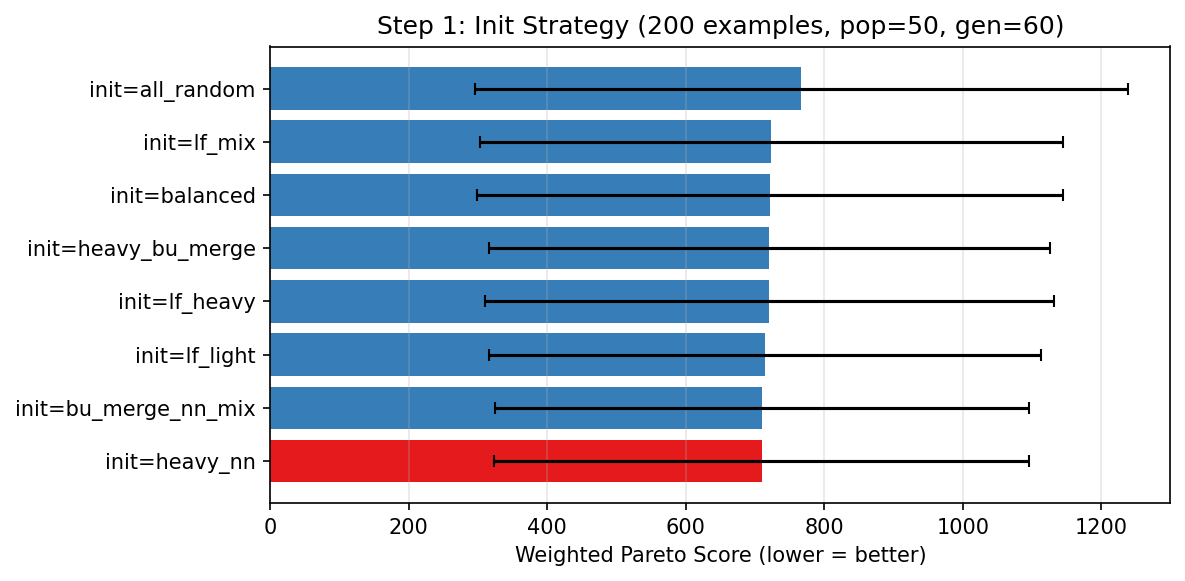
\includegraphics[width=0.8\textwidth]{figures/tune_init.png}
\caption{Init strategy comparison (200 examples, pop=50, gen=60).}
\end{figure}

\begin{table}[H]
\centering
\begin{tabular}{lcc}
\toprule
\textbf{Init} & \textbf{WPS} & \textbf{Composition} \\
\midrule
\textbf{heavy\_nn} & \textbf{709 $\pm$ 386} & 50\% nearest-neighbor + 30\% bottom-up merge + 10\% random + 10\% top-down \\
bu\_merge\_nn\_mix & 709 $\pm$ 386 & 40\% bottom-up merge + 30\% NN + 10\% GNN + 10\% each \\
lf\_light & 714 $\pm$ 399 & 30\% NN + 30\% BU merge + 10\% largest-first + 10\% GNN + rest \\
lf\_heavy & 721 $\pm$ 411 & 50\% largest-first + 20\% BU merge + 15\% NN + rest \\
all\_random & 767 $\pm$ 471 & 100\% random \\
\bottomrule
\end{tabular}
\end{table}

\subsection{Step 2: Mutation Strategy}

\begin{figure}[H]
\centering
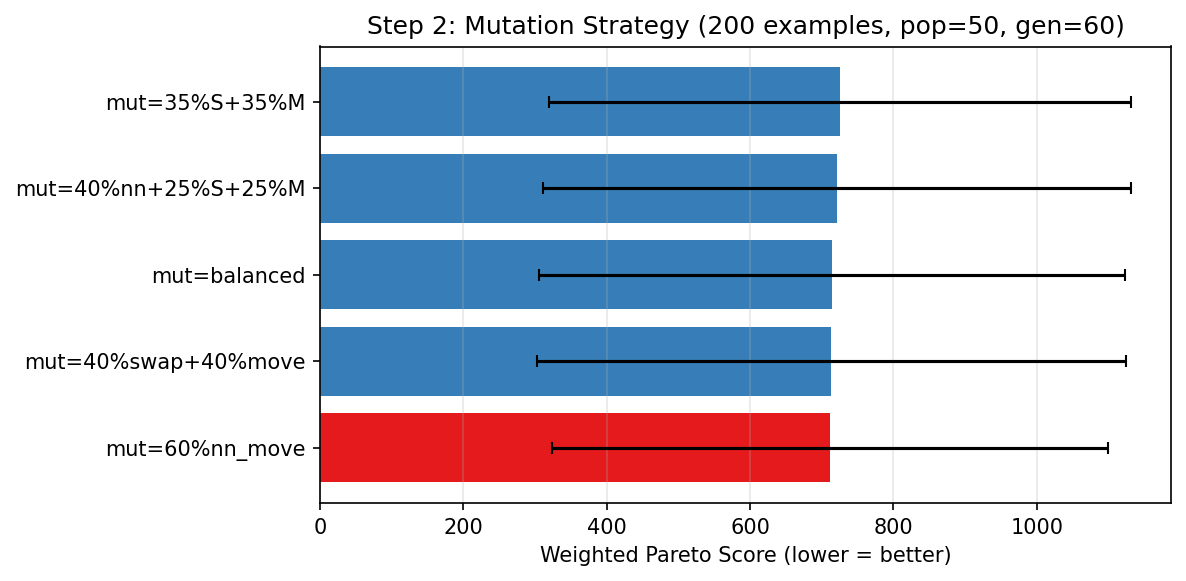
\includegraphics[width=0.8\textwidth]{figures/tune_mutation.png}
\caption{Mutation strategy comparison.}
\end{figure}

\begin{table}[H]
\centering
\begin{tabular}{lcc}
\toprule
\textbf{Mutation} & \textbf{WPS} & \textbf{Composition} \\
\midrule
\textbf{60\%nn\_move} & \textbf{712 $\pm$ 387} & 60\% nn-move + 15\% split + 15\% merge + 5\% swap + 5\% move \\
40\%swap+40\%move & 713 $\pm$ 411 & 40\% swap + 40\% move + 5\% split + 5\% merge + 10\% nn-move \\
balanced & 715 $\pm$ 409 & 20\% each \\
40\%nn+25\%S+25\%M & 721 $\pm$ 410 & 40\% nn-move + 25\% split + 25\% merge \\
35\%S+35\%M & 725 $\pm$ 406 & 35\% split + 35\% merge \\
\bottomrule
\end{tabular}
\end{table}

Top 3 are within 0.3\%.  Smart crossover repair handles table-count exploration, freeing mutations for local optimization.

\subsection{Step 3: Population Size}

\begin{figure}[H]
\centering
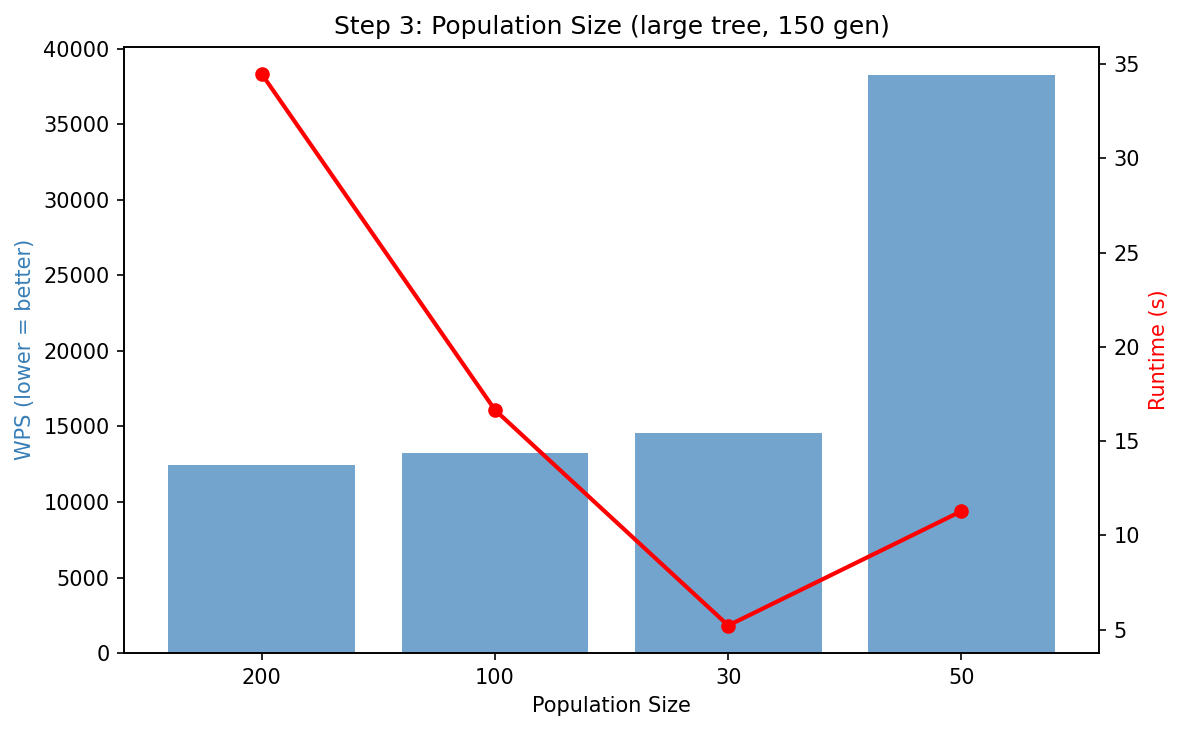
\includegraphics[width=0.7\textwidth]{figures/tune_popsize.png}
\caption{Population size: quality (bars) vs runtime (line).  Large tree, 150 gen.}
\end{figure}

\begin{table}[H]
\centering
\begin{tabular}{lccc}
\toprule
\textbf{Pop} & \textbf{WPS} & \textbf{Time} \\
\midrule
\textbf{200} & \textbf{12,463} & 34s \\
100 & 13,221 & 17s \\
30 & 14,580 & 5s \\
50 & 38,240 & 11s \\
\bottomrule
\end{tabular}
\end{table}

\subsection{Step 4: Convergence}

\begin{figure}[H]
\centering
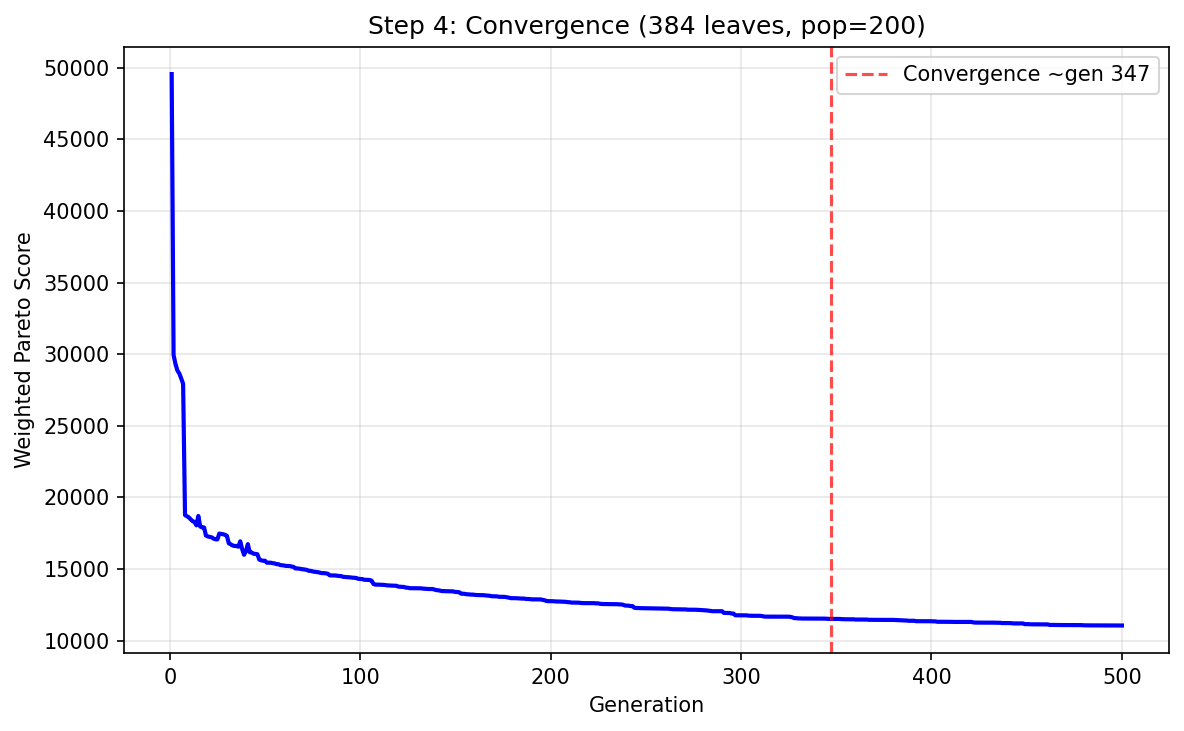
\includegraphics[width=0.7\textwidth]{figures/tune_convergence.png}
\caption{WPS over 500 generations.  Red line: convergence ($<0.5\%$ improvement over 20 gen).}
\end{figure}

Convergence at \textbf{generation 347}.  Final WPS = 11,054.

%=================================================================
\section{Results: Large-Scale Benchmark}
%=================================================================

Best config from tuning: init=heavy\_nn (50\% nearest-neighbor, 30\% bottom-up merge, 10\% each random/top-down), mutation=60\%nn\_move, pop=200, 500 gen.  Tree: 384 leaves, 978 people, $C=10$, min 98 tables.  Generated by \texttt{run\_all.py} with \texttt{generate\_synthetic\_tree(800, max\_group\_size=4, max\_children=4, seed=42)}.

\textbf{Note}: the recommended production config (Section~8) adds 10\% \texttt{largest\_first} to ensure min-table reachability on hard instances, at no WPS cost.

\begin{figure}[H]
\centering
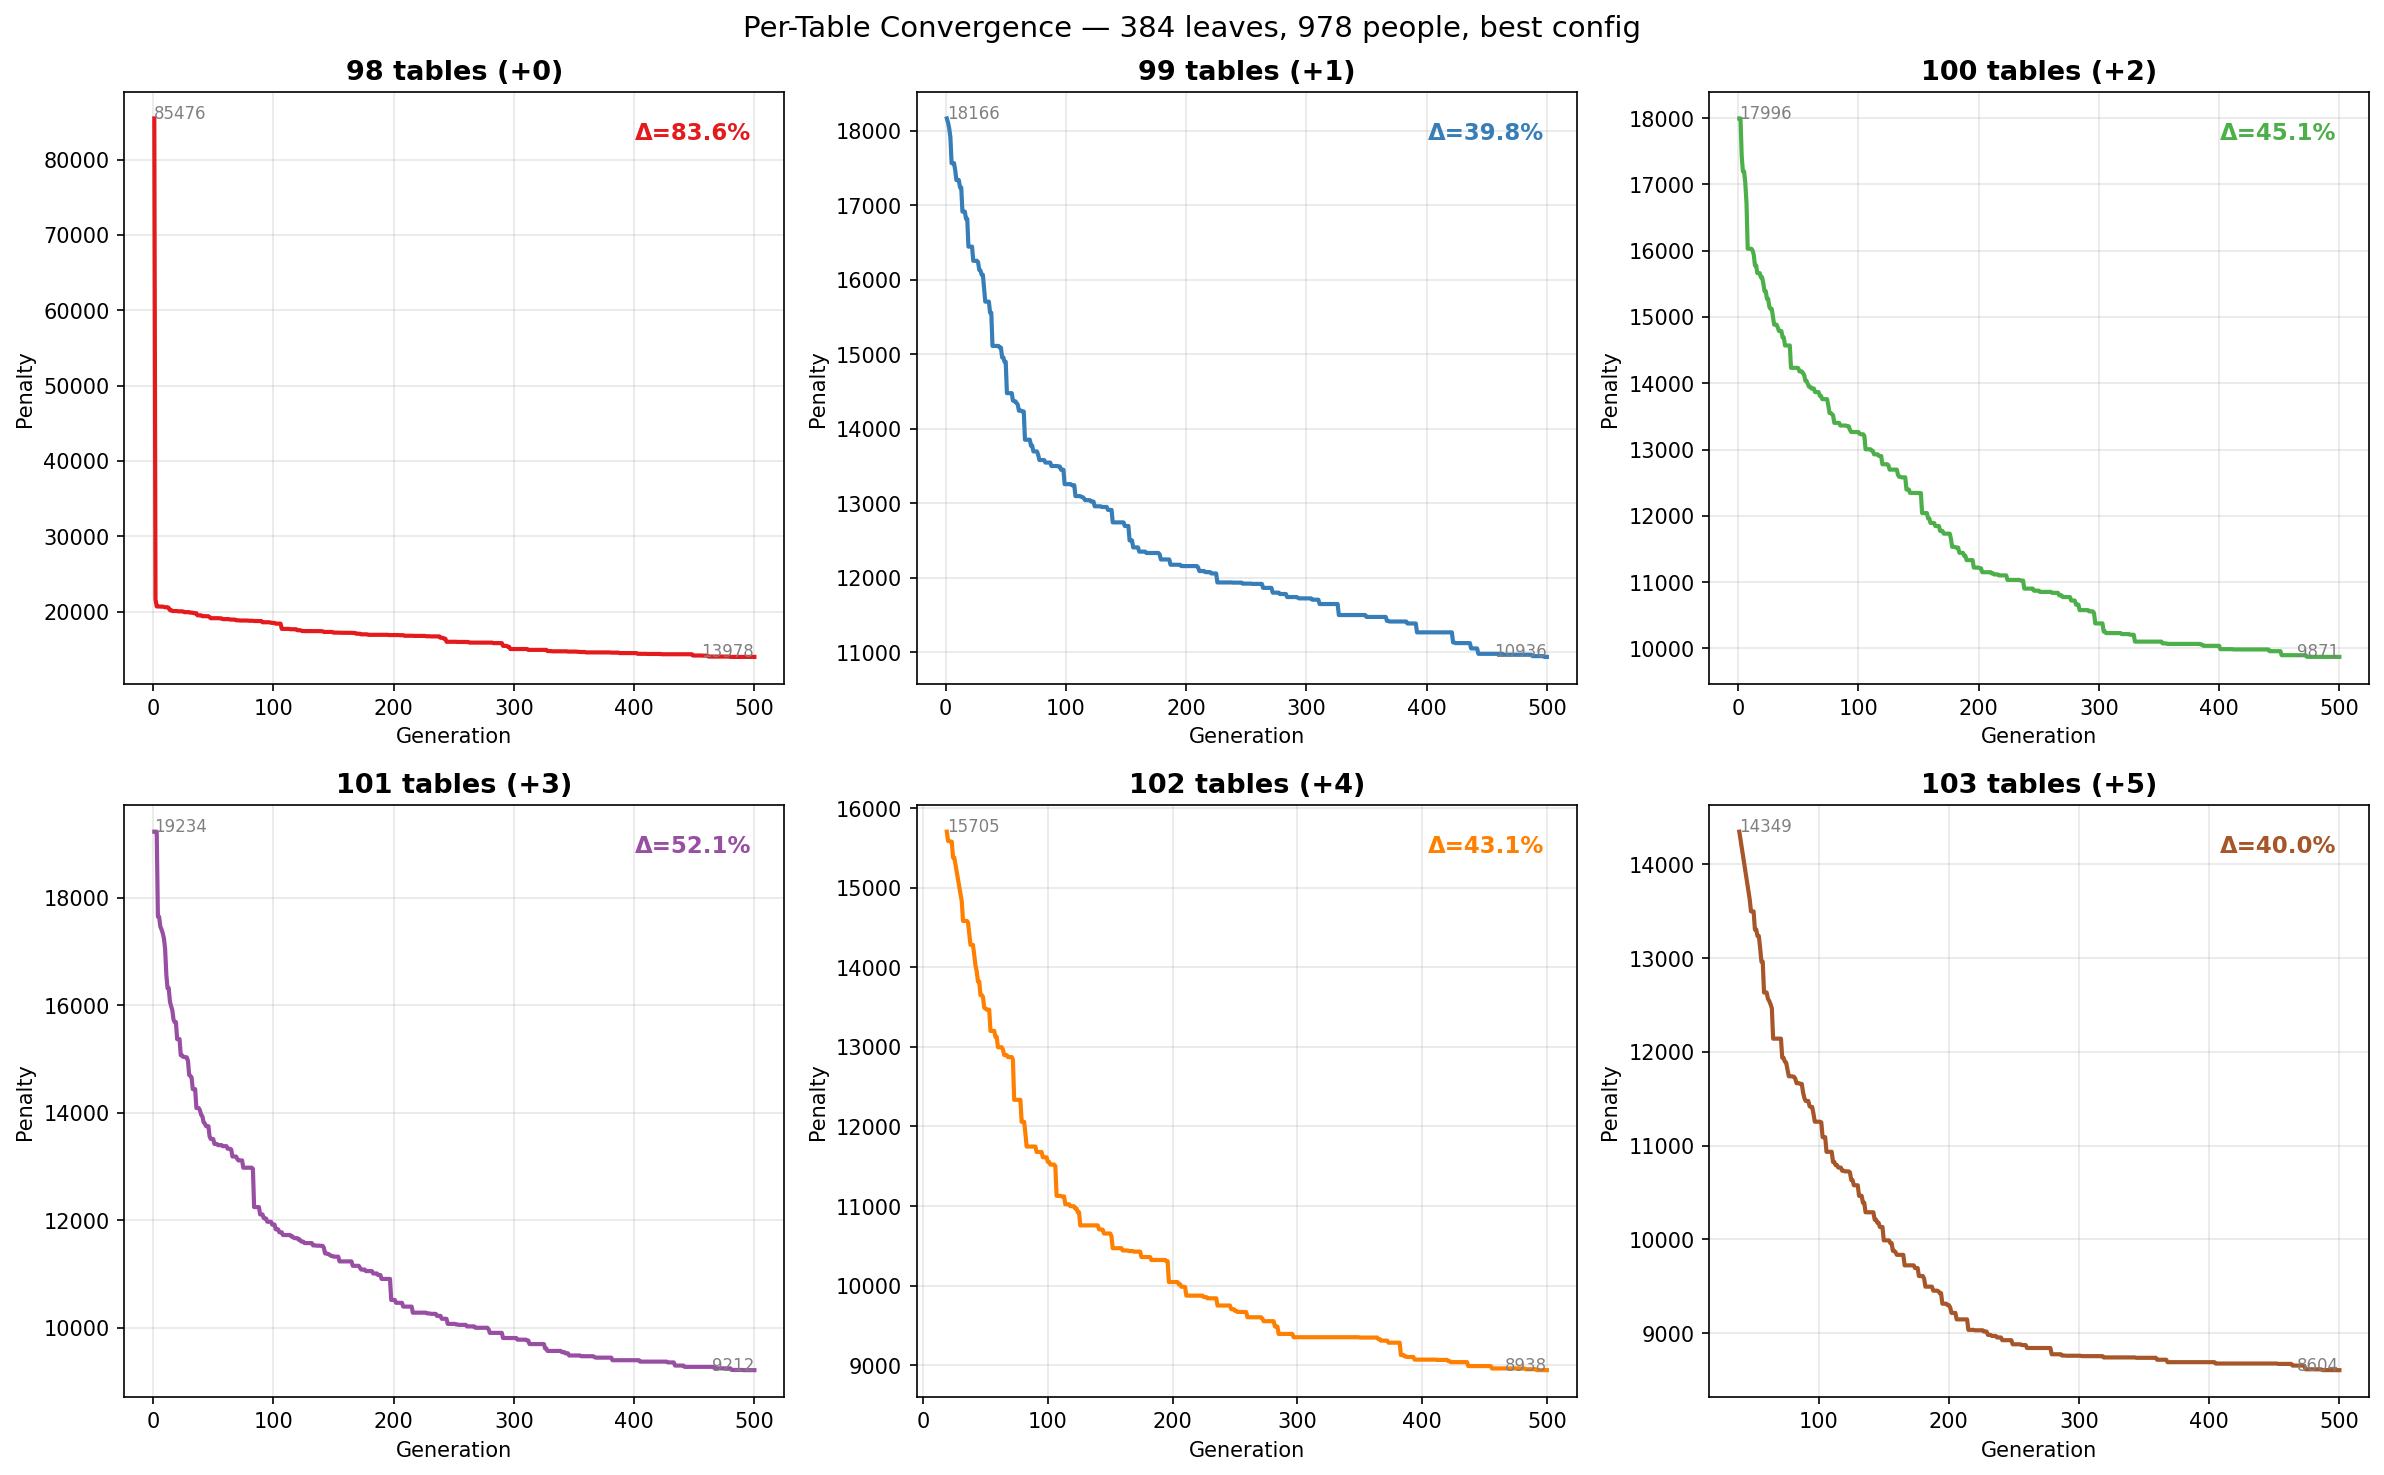
\includegraphics[width=0.95\textwidth]{figures/results_per_table.png}
\caption{Penalty convergence per table count (98--103).}
\end{figure}

\begin{table}[H]
\centering
\caption{Final penalty per table count after 500 generations.}
\begin{tabular}{lcc}
\toprule
\textbf{Tables} & \textbf{Penalty} & \textbf{Note} \\
\midrule
98 (min) & 13,978 & Hardest to optimize \\
99 (+1) & 10,936 & 22\% better than 98 \\
100 (+2) & 9,871 & \\
101 (+3) & 9,212 & \\
102 (+4) & 8,938 & \\
103 (+5) & 8,604 & Best quality \\
\bottomrule
\end{tabular}
\end{table}

Runtime: 109s for 500 gen (convergence at gen $\sim$347).

%=================================================================
\section{GNN Evaluation}
\label{sec:gnn-results}
%=================================================================

Using the same large tree from Section~6 (384 leaves, 978 people, $C=10$), we evaluate adding 10\% GNN to the init mix.  Baseline: the best init without GNN (nearest-neighbor heavy).  Both use pop=100, 150 generations, 30 runs each with a two-sided t-test.  Two outlier runs per group (penalty $>70{,}000$, caused by EA getting stuck) were excluded via IQR filtering.

\begin{table}[H]
\centering
\begin{tabular}{lcccc}
\toprule
\textbf{Config} & \textbf{Penalty@min} & \textbf{Std} & \textbf{Runs} & \textbf{vs no GNN} \\
\midrule
No GNN & 15,964 & $\pm$ 1,162 & 28/30 & baseline \\
\textbf{10\% GNN in init} & \textbf{15,113} & $\pm$ \textbf{898} & 28/30 & \textbf{+5.3\%} \\
\bottomrule
\end{tabular}
\end{table}

\textbf{Statistical significance}: $t=3.01$, $p=0.004$ (significant at 1\%).  The GNN improves penalty at minimum tables by 5.3\% and reduces variance (lower std).  The GNN rarely hits the minimum table count on its own (0.8\% vs 3.8\% for nearest-neighbor), but when included in the init mix, it provides diverse seeds that the EA exploits over subsequent generations.

\textbf{Init quality comparison} (500 samples, no EA):
\begin{table}[H]
\centering
\begin{tabular}{lccc}
\toprule
\textbf{Method} & \textbf{Hit min tables} & \textbf{Penalty@min} & \textbf{Time/sample} \\
\midrule
random & 91.8\% & 93,053 & 6.6\,ms \\
nearest-neighbor & 3.8\% & 20,422 & 36\,ms \\
top-down & 92.0\% & 93,089 & 111\,ms \\
bottom-up merge & 93.2\% & 92,983 & 28\,ms \\
GNN & 0.8\% & 21,275 & 154\,ms \\
\bottomrule
\end{tabular}
\end{table}

Nearest-neighbor produces the best standalone init quality by far.  Random, top-down, and bottom-up merge hit min tables often but with very poor penalty ($\sim$93k) because they don't optimize for cohesion.  The GNN's value emerges only within the EA, not as a standalone initializer.

\textbf{Mid-run injection} (Section~4.6) disrupts convergence in practice and performs worse than init-only seeding.  Init-only seeding is recommended.

\textbf{Transfer learning} (Section~4.4) requires an initial EA solve to generate finetuning targets, negating the time savings.  Not recommended as a standalone technique.

%=================================================================
\section{Recommended Defaults}
%=================================================================

\begin{table}[H]
\centering
\begin{tabular}{ll}
\toprule
\textbf{Parameter} & \textbf{Value} \\
\midrule
Init mix & 40\% nearest-neighbor + 20\% bottom-up merge + 10\% largest-first + 10\% GNN + 10\% random + 10\% top-down \\
Mutation & 60\% nn-move + 15\% split + 15\% merge + 5\% swap + 5\% move \\
Population & 200 (or 100 for 2$\times$ faster) \\
Generations & 250 (converges by $\sim$gen 347) \\
$\alpha, p$ & 2.0, 2.0 \\
$\Delta$ & 5 \\
\bottomrule
\end{tabular}
\end{table}

Expected runtime for 400 leaves: $\sim$100s (pop=200) or $\sim$50s (pop=100).

%=================================================================
\section{Key Takeaways}
%=================================================================

\begin{enumerate}
\item \textbf{Nearest-neighbor is the best WPS initializer} (50\% allocation wins on WPS), but \textbf{largest-first is essential for min-table reachability} on hard instances.  The recommended config includes 10\% largest-first at no WPS cost.
\item \textbf{Nearest-neighbor move dominates mutations} (60\%) because smart crossover fragment repair handles table-count exploration, freeing mutations for local optimization.
\item \textbf{All-random init is 8\% worse} on small trees and fails on large trees.
\item \textbf{Pop=200 is optimal}; pop=100 is the speed/quality sweet spot.
\item \textbf{GNN improves penalty by 5.3\% ($p=0.004$)} at 10\% of the init mix.  Trained on min-table EA targets with subtree-people features; acts as a tiebreaker via blended distance ($\alpha=0.2$).
\item \textbf{Convergence at $\sim$gen 347} for 384 leaves.
\end{enumerate}

%=================================================================
\appendix
\section{Reproduction}
%=================================================================

\begin{lstlisting}
pip install numpy pymoo torch torch-geometric scipy matplotlib

# Reproduce GNN training + comparison (recommended)
python3.10 train_and_evaluate_gnn.py --step 1   # Train GNN (~47 min)
python3.10 train_and_evaluate_gnn.py --step 2   # Compare with/without GNN (~50 min)

# Full hyperparameter tuning pipeline (optional, ~2h)
python3.10 run_all.py

# Verify report examples and regenerate figures
python3.10 validate_examples.py
python3.10 generate_examples.py
\end{lstlisting}

\textbf{Note}: Step 2 requires \texttt{gnn\_model.pt} from Step 1.  If the file is absent, the GNN init slots fall back to random valid silently.  The optimizer also supports mid-run GNN injection via \texttt{gnn\_inject=True}, but this is not recommended (see Section~\ref{sec:gnn-results}).

\end{document}
